\documentclass{beamer}
\usepackage{../tut-slides}
\usepackage{../mathoperatorsAuD}

\usepackage{amsmath,amssymb}
\usepackage{enumerate}
%\usepackage[inline]{enumitem} 		%customize label
%\newcommand{\labelitemi}{\raisebox{1pt}{\scalebox{.9}{$\blacktriangleright$}}}
%\newcommand{\labelitemii}{$\vartriangleright$}
%\newcommand{\labelitemiii}{--}
\setbeamertemplate{itemize item}{\raisebox{1pt}{\scalebox{.9}{$\blacktriangleright$}}}
\setbeamertemplate{itemize subitem}{$\vartriangleright$}

\usepackage{booktabs}
\usepackage{tabularx}
\usepackage{tabu}
\newcommand*\head{\rowfont{\bfseries}}
\newcommand*{\tw}{\rowfont{\ttfamily}}
\renewcommand{\tabularxcolumn}[1]{>{\hspace{0pt}}m{#1}}

\usepackage{cancel}

%%%% EBNF-Terme %%%%
\newcommand{\wdh}[1]{\hat{\{} \ #1 \ \hat{\}}}
\newcommand{\opt}[2]{\hat{(} \ #1 \ \hat{|} \ #2 \ \hat{)}}
\newcommand{\byp}[1]{\hat{[} \ #1 \ \hat{]}}
\newcommand{\rdb}[1]{\hat{(} \ #1 \ \hat{)}}

\begin{document}	
	\title{Algorithmen und Datenstrukturen}
	\subtitle{Übung 2: Syntaxdiagramme}
	\author{Eric Kunze}
	\email{eric.kunze@mailbox.tu-dresden.de}
	\city{TU Dresden}
%	\institute{Lehrstuhl für Grundlagen der Programmierung}
	\titlegraphic{
\includegraphics[width=2cm]{../TUD-white.pdf}}
	\date{06.11.2019}

	\maketitle


%%%%%%%%%%%%%%%%%%%%%%%%%%%%%%%%%%%%%%%%%%%%%%%%%%%%%%%%%%%%%%%%%%%%%%%%%%%%%

\section{Syntaxdiagramme}

\begin{frame}
	\begin{itemize}
		\item syntaktische Variable = Nichtterminalsymbol = Name eines Syntaxdiagramms
		\item Jedes Kästchen ist mit dem Namen eines Syntaxdiagramms beschriftet.
		\item Jedes Oval ist mit einem Terminalsymbol beschriftet.
	\end{itemize}

	\pause

	\textbf{Rücksprungalgorithmus}
	\begin{itemize}
		\item jedes Kästchen bekommt eindeutige Marke (Rücksprungadresse)
		\item beim Betreten eines Syntaxdiagramms wird eine Marke auf den Keller gelegt
		\item Nachweis von Zugehörigkeit eines Wortes zu einer Sprache
	\end{itemize}
\end{frame}

\begin{frame} \frametitle{Aufgabe 1}
	\begin{itemize}
		\item Teil (a) ---
		z.B. $\epsilon, a, c, caa, aaaa, \dots$
		\item Teil (b) ---
		z.B. $aaac, abacac, abbaccac, \dots$
		\item 	Teil (c) ---
		z.B. $\epsilon, ab, abab, ac, aabcab, \dots$
	\end{itemize}
\end{frame}

\begin{frame} \frametitle{Aufgabe 2 --- Teil (a)}
	\begin{align*}
		L &= \menge{a^{2i} c b^{3i} c^k d^{2k+1} \mid i > 0, k \ge 0} \\
		&= \menge{a^{2i} c b^{3i} \mid i > 0} * \menge{c^k d^{2k+1} \mid k \ge 0}
	\end{align*}
	
	\centering
	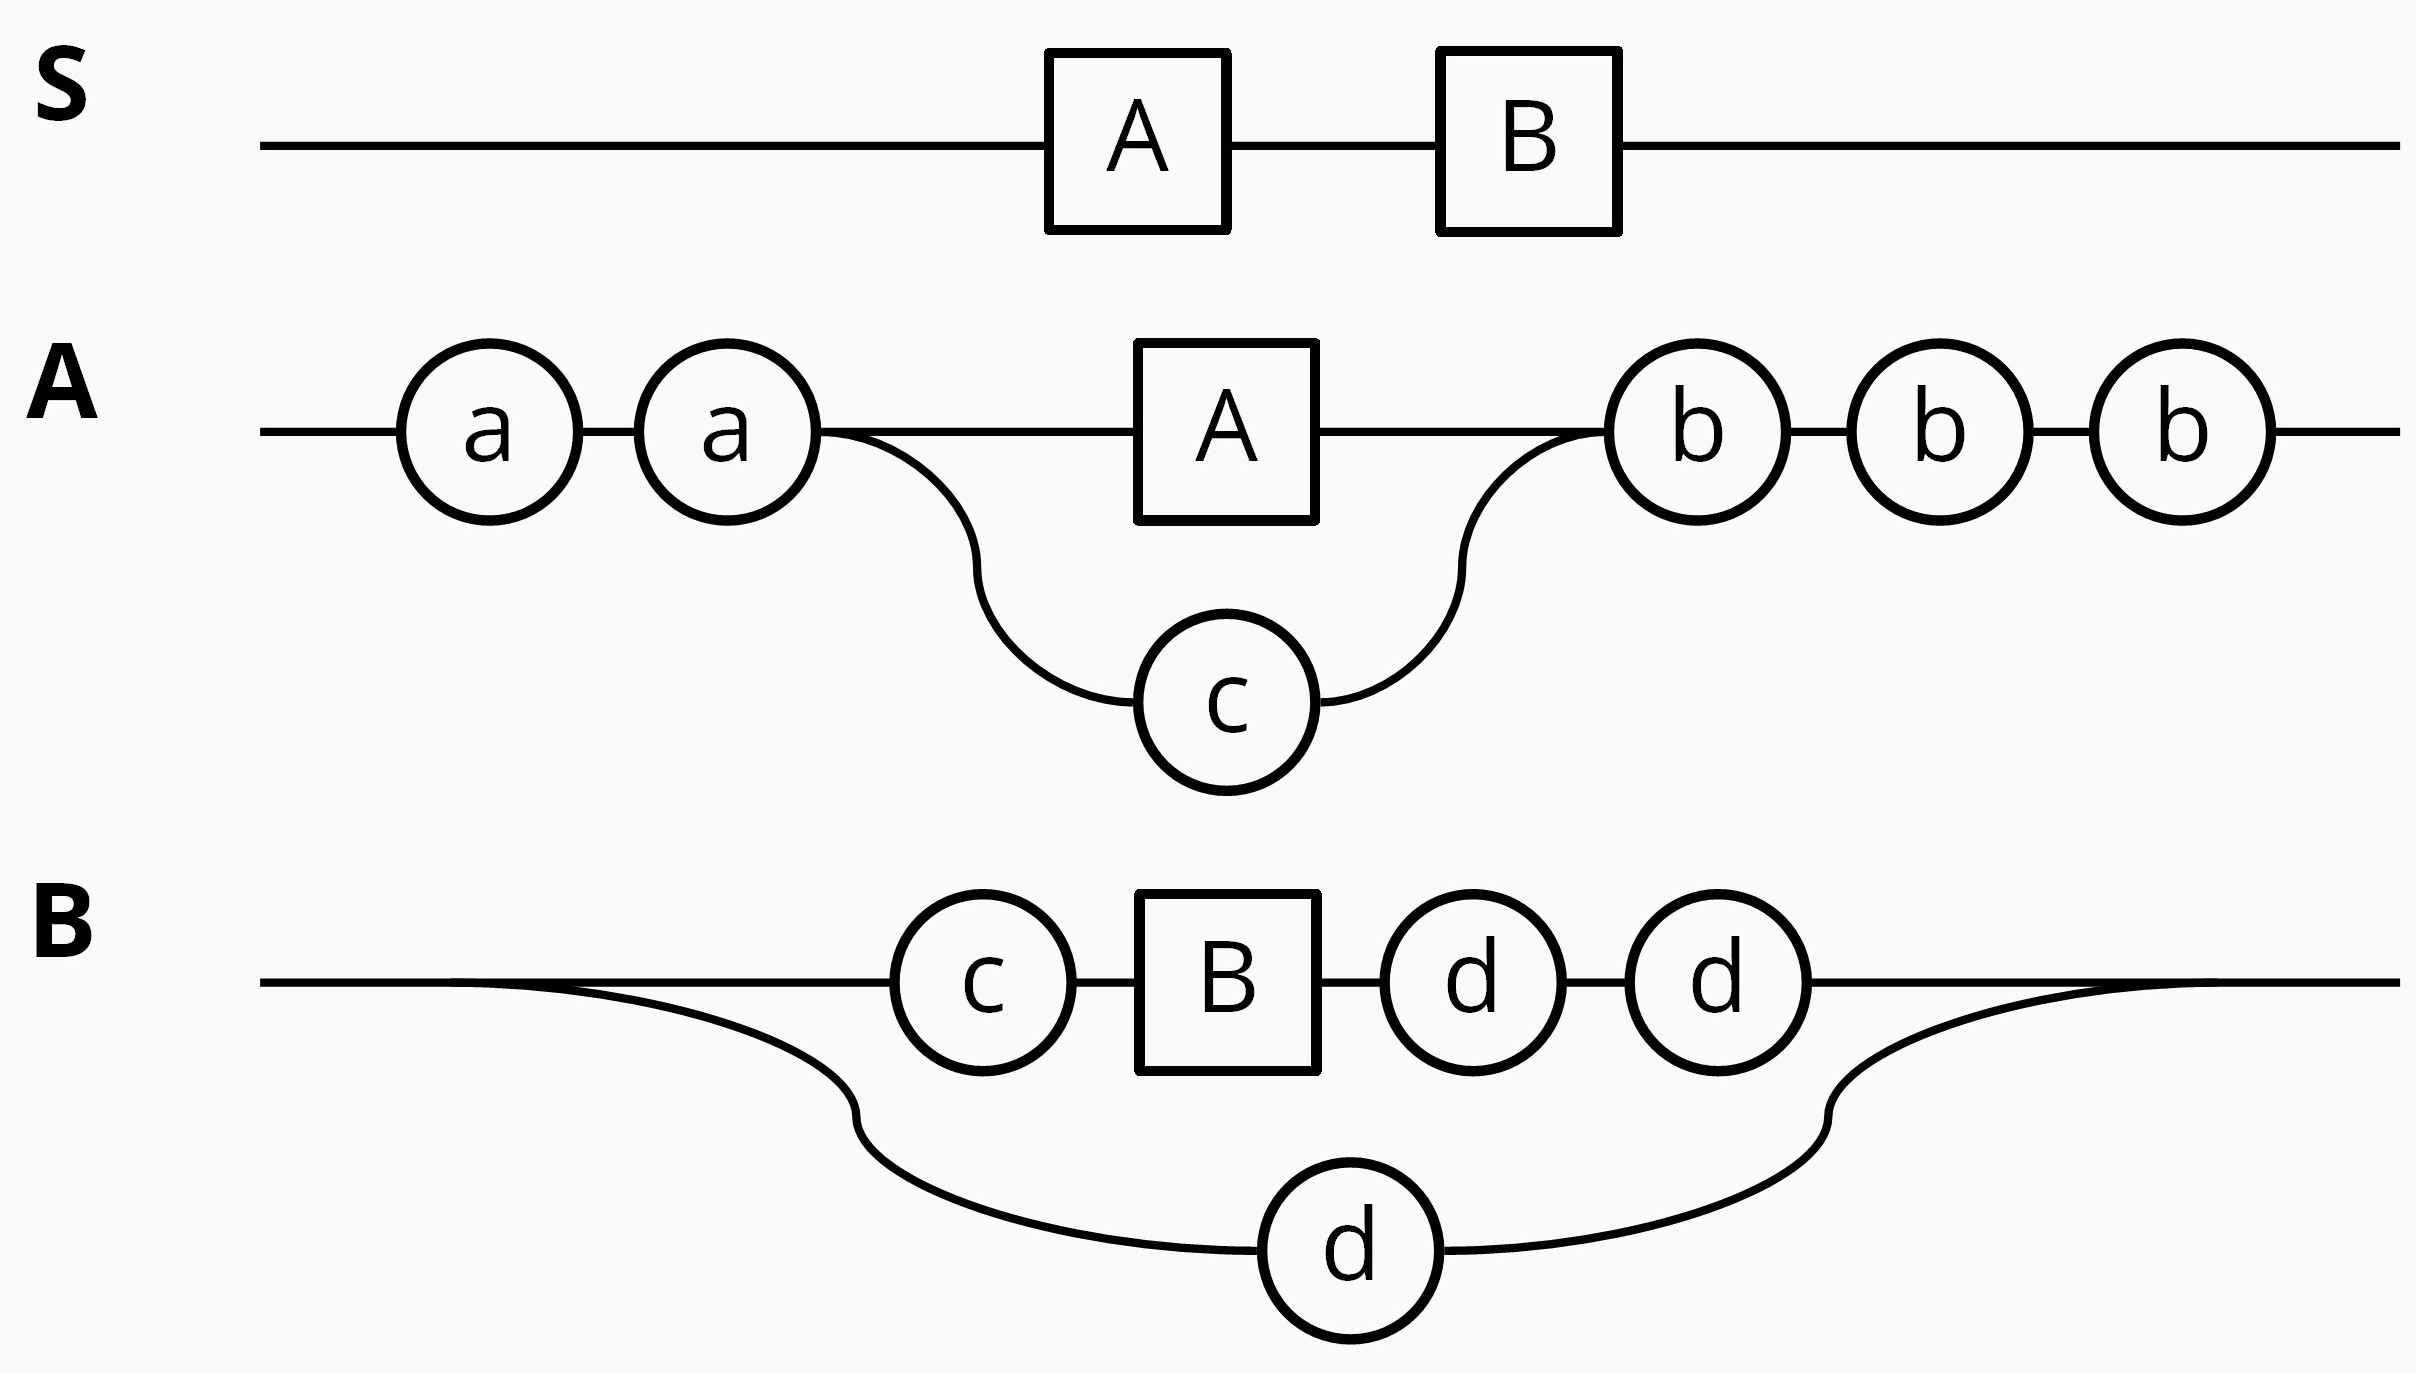
\includegraphics[width=.9\textwidth]{tut02_syntax_dia_2a.jpg}
\end{frame}

\begin{frame} \frametitle{Aufgabe 2 --- Teil (b)}
	\begin{minipage}{\dimexpr0.5\linewidth-\fboxrule-\fboxsep}
		\small
		\textbf{Protokollierungszeitpunkte:}
		\begin{itemize}
			\item jeder Aufenthalt in einem Syntaxdiagramm entspricht einer Zeile
			\item jede Zeile führt eine Operation auf dem Markenkeller aus
			\item $\cancel{3}$ = Rücksprung zu Marke $3$
		\end{itemize}
	\end{minipage}
	\pause
	\begin{minipage}{\dimexpr0.5\linewidth-\fboxrule-\fboxsep}
		\centering
		\begin{tabular}{l|r}
			\hline
			Wort & Markenkeller \\ \hline \pause
			a & 1 \\ \pause
			a & 31 \\ \pause
			aa & 131 \\ \pause
			aaa & 2131 \\ \pause
			aaa & 32131 \\ \pause
			aaaaccb & $\cancel{3} 2131$ \\ \pause
			aaaaccb & $\cancel{2}131$ \\ \pause
			aaaaccbd & $\cancel{1}31$ \\ \pause
			aaaaccbdb & $\cancel{3}1$ \\ \pause
			aaaaccbdb & $\cancel{1}$ \\ \pause
			aaaaccbdbb & -- \\ \hline
		\end{tabular}
	\end{minipage}

\end{frame}

\begin{frame} \frametitle{Aussagenlogik}
	\begin{block}{Alphabet der Aussagenlogik}
		Ein Alphabet der Aussagenlogik besteht aus
		\begin{itemize}
			\item einer (abzählbar) unendlichen Menge $\mathcal{R} = \menge{p_1,p_2,p_3, \dots}$ von aussagenlogischen Variablen
			\item der Menge $\mathcal{J} = \menge{\lnot, \land, \lor, \to, \leftrightarrow}$ von Junktoren
			\item der Menge $\menge{(,)}$ der Sonderzeichen.
		\end{itemize}
	\end{block}
	Wir beschränken uns im Folgenden auf die Junktoren $\mathcal{J} = \menge{\lnot, \lor}$ und die Variablen $p$ und $q$.
\end{frame}

\begin{frame}% \frametitle{Aussagenlogische Formeln}
	\begin{block}{Aussagenlogische Formeln}
		Die Menge von Formeln ist die \emph{kleinste} Menge $\mathcal{L}(\mathcal{R})$ von Zeichenreihen über $\mathcal{R}$, den Junktoren und den Sonderzeichen, die die folgenden Eigenschaften erfüllt:
		\begin{itemize}
			\item Wenn $F \in \mathcal{R}$, dann ist $F \in \mathcal{L}(\mathcal{R})$
			\item Wenn $F \in \mathcal{L}(\mathcal{R})$, dann ist $\lnot F \in \mathcal{L}(\mathcal{R})$
			\item Wenn $\circ \in \mathcal{J}$ ein zweistelliger Junktor ist und $F,G \in \mathcal{L}(\mathcal{R})$ sind, dann ist $(F \circ G) \in \mathcal{L}(\mathcal{R})$.
		\end{itemize}
	
		Da im Folgenden stets $\mathcal{J} = \menge{\lnot, \lor}$ gilt, und $\lor$ der einzige zweistellige Junktor ist, vereinfacht sich die dritte Bedingung zu:
		\begin{itemize}
			\item Wenn $F,G \in \mathcal{L}(\mathcal{R})$ sind, dann ist $(F \lor G) \in \mathcal{L}(\mathcal{R})$.
		\end{itemize}
	\end{block}
\end{frame}

\begin{frame} \frametitle{Aufgabe 3}
	\centering
	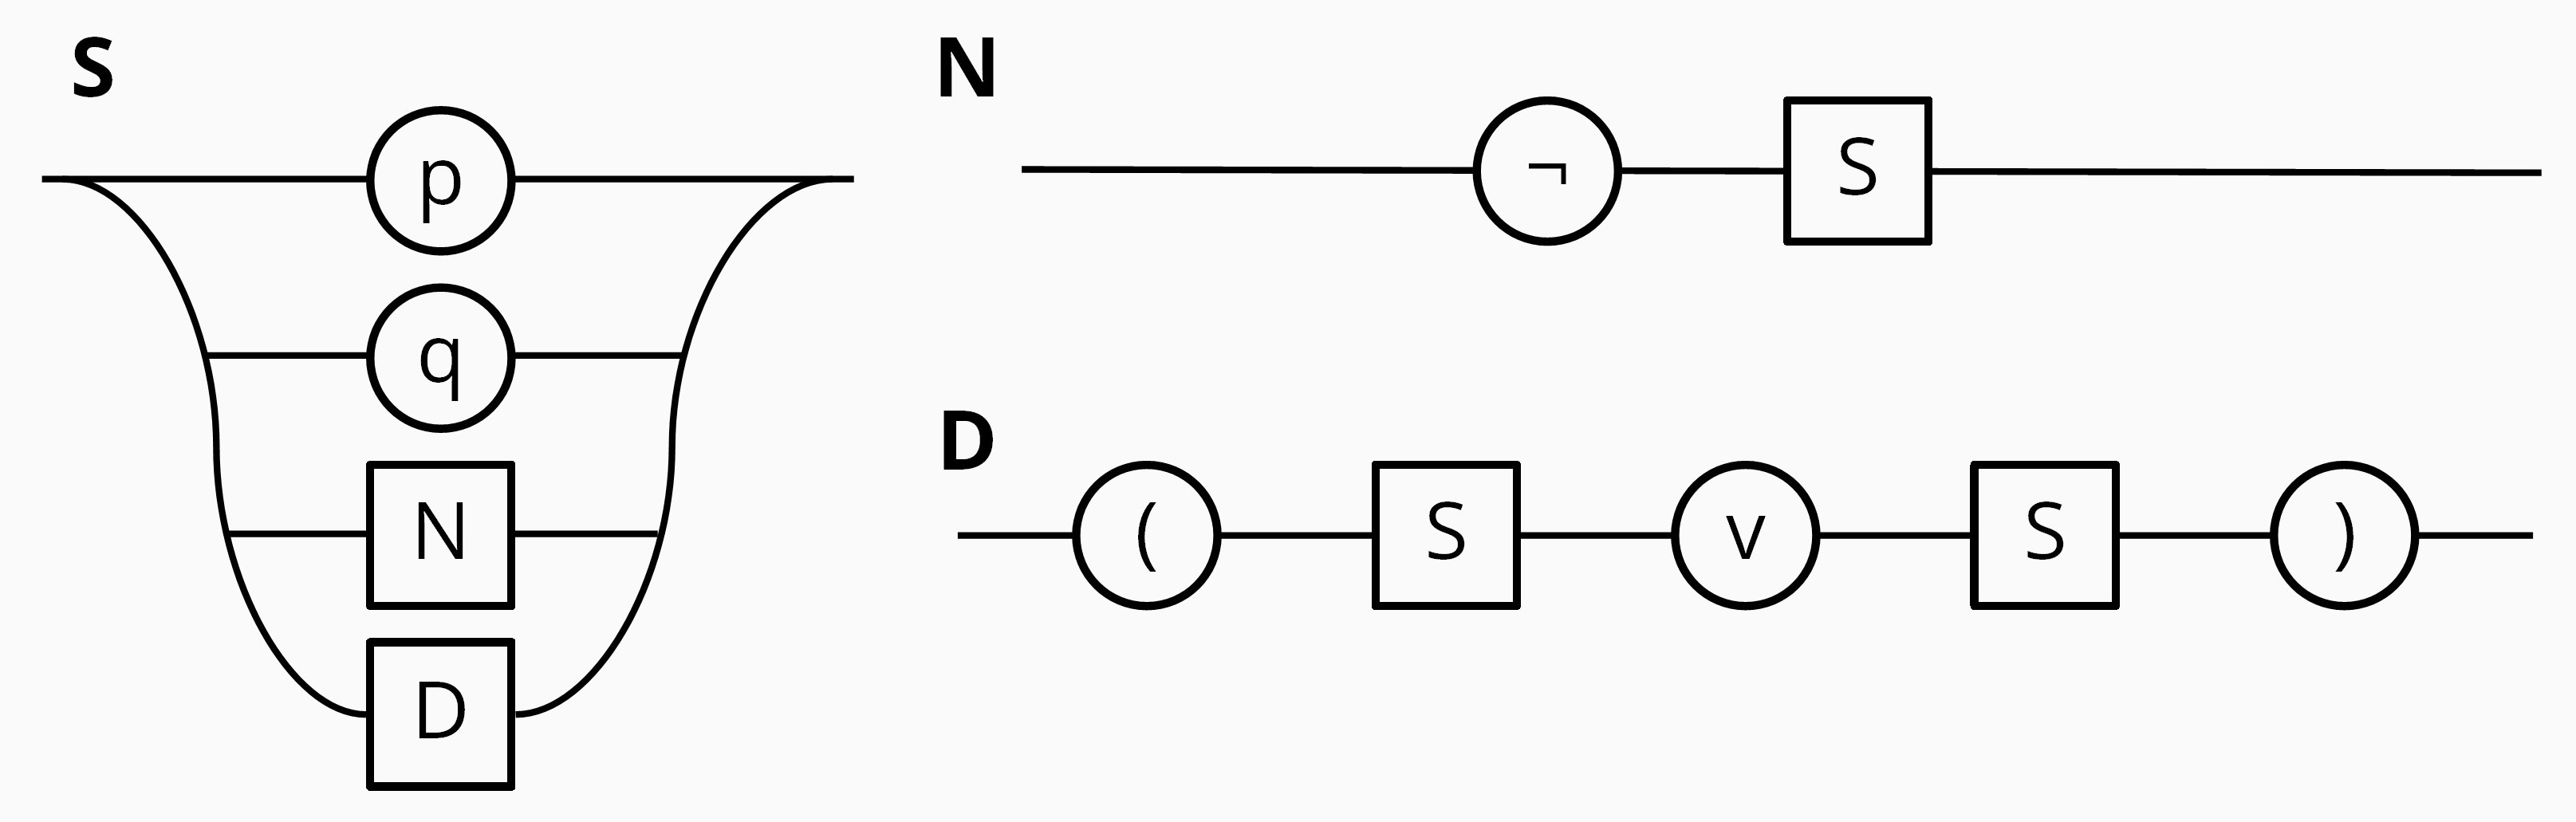
\includegraphics[width=\textwidth]{tut02_syntax_dia_3.jpg}
\end{frame}

\section{Extended Backus-Naur-Form}

\begin{frame} \frametitle{EBNF-Definition}
	\small
	\begin{itemize}
		\item EBNF-Definition besteht aus endlicher Menge von EBNF-Regeln.
		\item Jede EBNF-Regel besteht aus einer linken und einer rechten Seite, die rechte Seite ist ein EBNF-Term.
	\end{itemize}
	\pause
	\begin{block}{Definition: EBNF-Term}
		Seien $V$ eine endliche Menge (syntaktische Variablen) und $\Sigma$ eine endliche Menge (Terminalsymbole) mit $V \cap \Sigma = \emptyset$. Die Menge der EBNF-Terme über $V$ und $\Sigma$ (notiere: $T(\Sigma, V)$), ist die \emph{kleinste} Menge $T \subseteq \brackets{V \cup \Sigma \cup \menge{\hat{\{}, \hat{\}}, \hat{[}, \hat{]}, \hat{(}, \hat{)}, \hat{|}}}$ mit $V \subseteq T$, $\Sigma \subseteq T$ und
		\begin{itemize}
			\item Wenn $\alpha \in T$, so auch $\rdb{\alpha} \in T$, $\wdh{\alpha} \in T$, $\byp{\alpha} \in T$.
			\item Wenn $\alpha_1, \alpha_2 \in T$, so auch $\opt{\alpha_1}{\alpha_2} \in T$, $\alpha_1 \alpha_2 \in T$
		\end{itemize}
	\end{block}
	
\end{frame}

\begin{frame} \frametitle{Aufgabe 4}
	\renewcommand{\theenumi}{\bfseries\alph{enumi}}
	
	Sei $V = \menge{A,B}$ und $\Sigma = \menge{a,b,c,d}$.
	
	\begin{enumerate}
		\item $\wdh{A} \pause \in T(\Sigma,V)$ \pause
		\item $\wdh{\byp{B}} \pause \in T(\Sigma,V)$ \pause
		\item $\wdh{\opt{\byp{B}}{C}} \pause \notin T(\Sigma,V)$, da $C \notin V$ \pause
		\item $\byp{\opt{a}{B \cup \menge{c}}} \pause \notin T(\Sigma,V)$, da $\cup$ nicht in EBNF vorhanden \pause
		\item $\wdh{\opt{\byp{c}}{\opt{a}{b} a}} \pause \in T(\Sigma,V)$ \pause
		\item $c \wdh{\byp{A \hat{|} B}} \hat{]} \hat{|} d \pause \notin T(\Sigma,V)$, da $\hat{(}$ und $\hat{)}$ zu $\hat{|}$ fehlen \pause
		\item $\byp{\opt{a}{b}^\ast \ \hat{|} \ ABA} \pause \notin T(\Sigma,V)$, da ${}^\ast$ nicht in EBNF vorhanden
	\end{enumerate}
\end{frame}


\end{document}